En esta sección el objetivo será comparar todos los algoritmos diseñados e implementados en este trabajo.

A continuación incluiremos dos gráficos. Uno para poder observar como se comportan tanto nuestros algoritmos ante la familia de grafos \emph{3-caminos} y otro ante la familia \emph{3-caminos con puentes}.

\begin{figure}[H]
    \begin{minipage}{0.5\linewidth}
      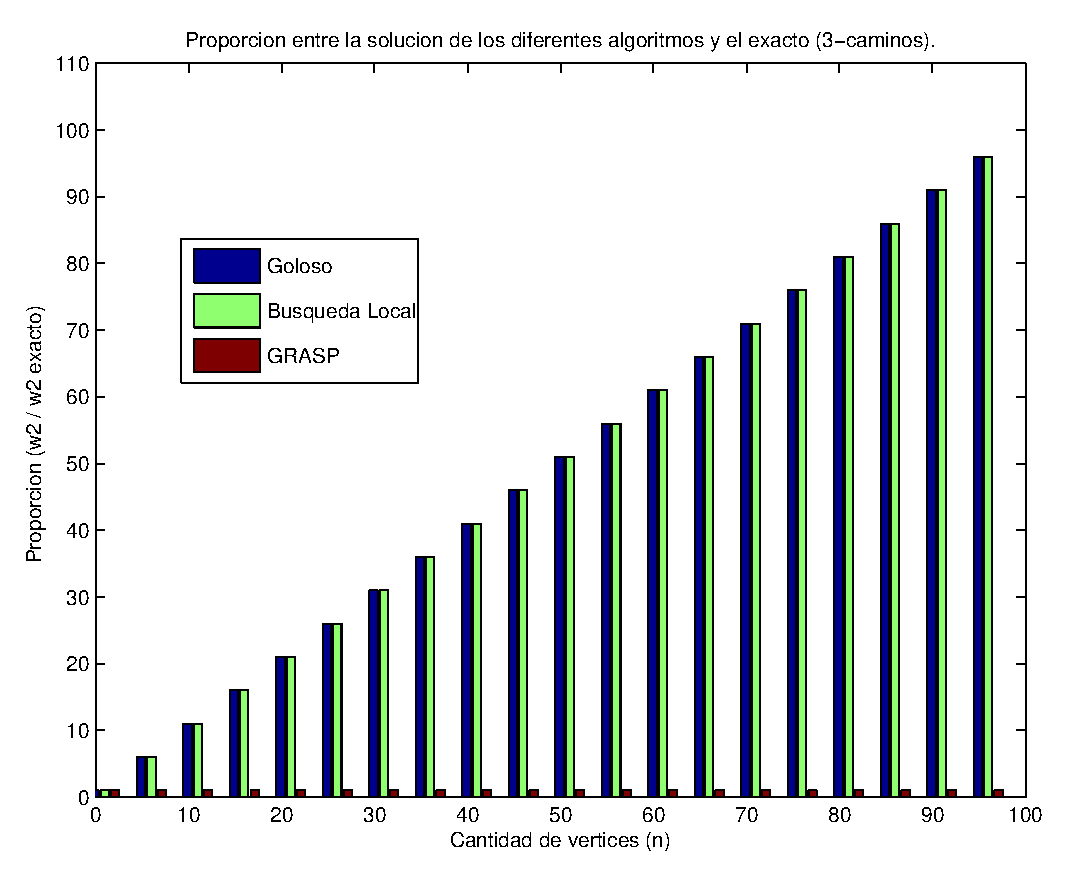
\includegraphics[width=\linewidth]{graficos/todos_proporcion_3caminos.eps}
      \caption{Comportamiento ante familia \emph{3-caminos}}\label{fig:comportamiento-familia-rompe}
    \end{minipage}
    \hfill
    \begin{minipage}{0.5\linewidth}
      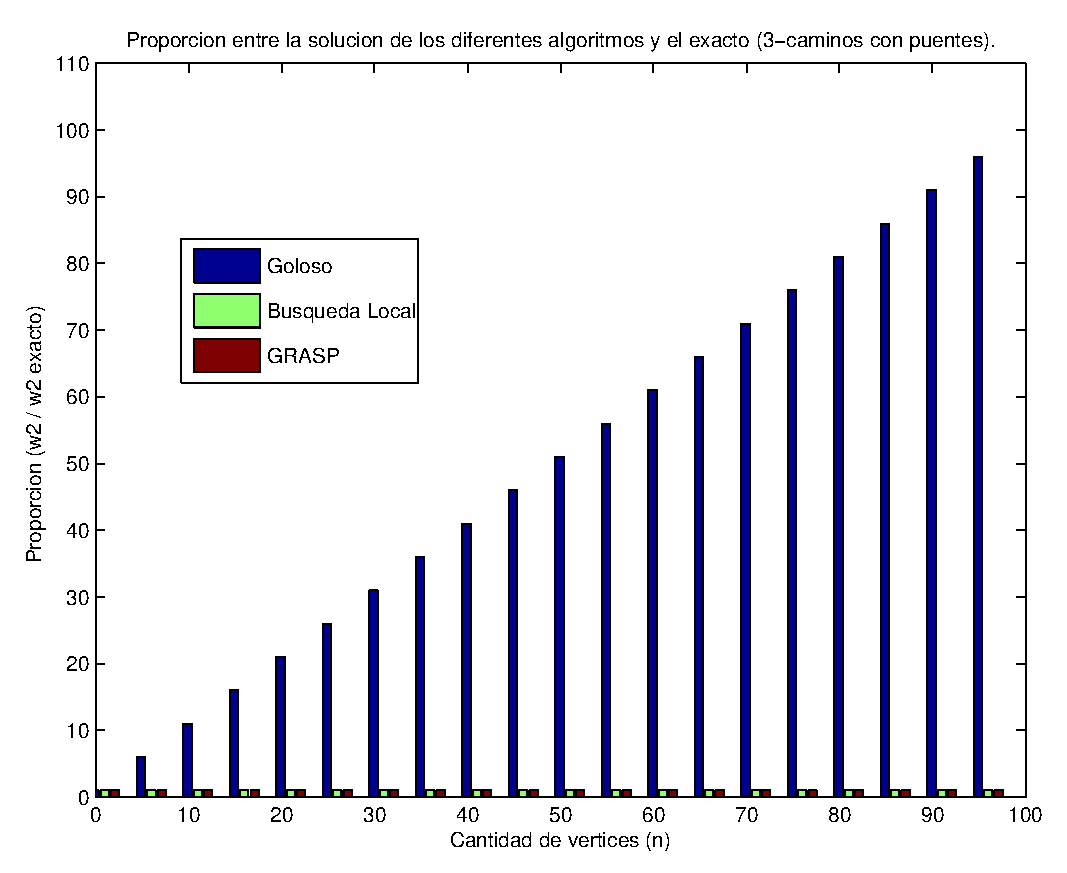
\includegraphics[width=\linewidth]{graficos/todos_proporcion_puentes.eps}
      \caption{Idem familia \emph{3-caminos con puentes}}\label{fig:comportamiento-familia-puente}
    \end{minipage}    
\end{figure}

En estos gráficos mostramos el comportamiento de tanto de los siguientes algoritmos para dos famlias de grafos. Los algoritmos medidos son los siguientes (todos en proporción al algoritmo exacto):

\begin{itemize}
 \item Algoritmo Goloso implementado en el trabajo
 \item Algoritmo de búsqueda local con algoritmo goloso como semilla
 \item Algoritmo GRASP que utiliza nuestro algoritmo goloso aleatorio y nuestro algoritmo de búsqueda local
\end{itemize}

Vale aclarar que todas las soluciones se muestran en proporción a las del algoritmo exacto.

En el gráfico de la Figura \ref{fig:comportamiento-familia-rompe} podemos ver que para los grafos de la familia \emph{3-caminos} nuestro algoritmo GRASP logra mejorar las soluciones del nuestro algoritmo goloso y de nuestro algoritmo de búsqueda local. Más aún, no solo las mejora sino que devuelve la solución óptima. También podemos volver a ver que nuestro algoritmo de búsqueda local no logra mejorar la solución inicial que le da el algoritmo goloso para esta familia de grafos cuando éstos superan una determinada cantidad de nodos (en secciones previas observamos que dicha cantidad es $7$).

A su vez, en el gráfico de la Figura \ref{fig:comportamiento-familia-puente} podemos observar que nuestro algoritmo goloso devuelve malas soluciones para la familia de grafos \emph{3-caminos con puentes}, pero que el algoritmo de búsqueda local las logra mejorar, devolviendo una solución óptima. También podemos ver que el algoritmo GRASP también se comporta de manera óptima para los algoritmos de dicha familia.